\section{Spatial Filtering}
\begin{doublespace}
\begin{figure}[htbp]
	\centering
		\includegraphics[trim =6cm 7cm 6cm 4cm, clip,width=0.70\textwidth]{graphics/Spatial_filtering_antenna_example.pdf}
	\caption{Example of a spatial filtering scenario: Sender with 1 antenna and Receiver with 3 antennas (as ULA)}
	\label{fig:SPatial_filtering_antenna_example}
\end{figure}
$\vec{x}[n]=\mat{x_1[n]\\x_2[n]\\\svdots\\x_M[n]}=\sum\limits_{k=1}^{d}\vec{a}(\Theta_k)s_k[n]+\vec{\nu}[n]$\\
$\vec{a}(\Theta)=\mat{1\\e^{-j2\pi \frac{\Delta}{\lambda} \cos(\Theta)}\\e^{-j 2 \cdot 2\pi \frac{\Delta}{\lambda} \cos(\Theta)}\\\svdots\\e^{-j(M-1)2\pi \frac{\Delta}{\lambda} \cos(\Theta)}}$\\
$\vec{x}[n]=\underbrace{\mat{\vec{a}(\Theta_1)&\vec{a}(\Theta_2)&\shdots&\vec{a}(\Theta_d)}}_{\ma{A}\in\mathbb{C}^{M\times d}}\cdot\underbrace{\mat{s_1[n]\\s_2[n]\\\svdots\\s_d[n]}}_{\vec{s}[n]\in\mathbb{C}^{d\times 1}}+\underbrace{\vec{\nu}}_{\in\mathbb{C}^{M\times 1}}$\\
$\vec{x}[n]=\ma{A}\cdot \vec{s}[n]+\vec{\nu}[n]$\\
With:\\
\begin{tabular}{rl}
$\vec{x}[n]$: & Observation Snapshot\\
$\ma{A}$: & Steering Matrix\\
$\vec{s}[n]$: & Signal Vector\\
$\vec{\nu}[n]$:& Noise\\
\end{tabular}\\ \\
\textbf{Observation Matrix (Space/time):}\\
$\ma{X}:=\mat{\vec{x}[n]&\vec{x}[n+1]&\shdots&\vec{x}[n+N-1]}\in\mathbb{C}^{M\times N}$\\
$\ma{S}:=\mat{\vec{s}[n]&\vec{s}[n+1]&\shdots&\vec{s}[n+N-1]}\in\mathbb{C}^{d\times N}$\\
$\ma{\nu}:=\mat{\vec{\nu}[n]&\vec{\nu}[n+1]&\shdots&\vec{\nu}[n+N-1]}\in\mathbb{C}^{M\times N}$\\
N snapshots\\
\mybox{
$\ma{X}=\ma{A}\ma{S}+\ma{\nu}$
}\\  \\
\begin{tabular}{ll}
\underline{Given:}&\ma{X} and \ma{A}\\
&and possibly $2^{nd}$-order statistics of \ma{S} and/or $\ma{\nu}$\\
\underline{Find:}&Estimate $\ma{\hat{S}}$ of \ma{S}\\
\underline{Here:}&Linear estimations $\ma{\hat{S}}=\ma{W}^H\ma{X}$\\
\end{tabular}
\end{doublespace}

\subsection{Case 1: Only X and A are known - Least Square}
\begin{doublespace}
Idea: $\ma{X}\approx\ma{A}\ma{S}\qquad$ (we assume that \ma{\nu} is small)\\
$\ma{\hat{S}}=\arg \min\limits_{\ma{S}}||\ma{X}-\ma{A}\ma{S}||_F^2$\\
$\rightarrow$ Least squares solution\\
\begin{flalign*}
||\ma{B}||_F^2=\sum\limits_{n,m}|B_{n,m}|^2=\sum\limits_{k=1}^{M}\vec{b}_k^H\vec{b}_k=\sum\limits_{k=1}^{M}\abs{\abs{\vec{b}_k}}_2^2=\trace\ma{B}^H\ma{B}
=\trace \mat{\vec{b}_1^H\\\vec{b}_2^H\\\svdots}\mat{\vec{b}_1&\vec{b}_2&\shdots}=\vec{b}_1^H\vec{b}_1+\vec{b}_2^H\vec{b}_2+\shdots
\end{flalign*}
Frobenius norm of the error:
\begin{flalign*}
\varepsilon &= ||\ma{X}-\ma{A}\ma{S}||_F^2=\trace\left((\ma{X}-\ma{A}\ma{S})^H(\ma{X}-\ma{A}\ma{S})\right)
=\trace\left((\ma{X}^H-\ma{S}^H\ma{A}^H)(\ma{X}-\ma{A}\ma{S})\right)&&\\
&=\trace(\ma{X}\ma{X}^H)-\trace(\ma{X}^H\ma{A}\ma{S})-\trace(\ma{S}^H\underbrace{\ma{A}^H\ma{X}}_{\ma{B}})+\trace(\ma{S}^H\ma{A}^H\ma{A}\ma{S})
\end{flalign*}

\mybox{
\textbf{Definition}:  Derivation of a scalar function with respect to a matrix:\\
$\frac{\partial \varepsilon}{\partial \ma{S}^*}:=\mat{\frac{\partial \varepsilon}{\partial \vec{S}_1^*}&\frac{\partial \varepsilon}{\partial \vec{S}_2^*}&\shdots&\frac{\partial \varepsilon}{\partial \vec{S}_N^*}}$}\\
\ \\

\with substitution: $\ma{A}^H\ma{X}=\ma{B}$\\

$\frac{\partial\trace(\ma{S}^H\ma{B})}{\partial\vec{s}_i^*}=\frac{\partial\trace \mat{\vec{s}_1^H\\\svdots\\\vec{s}_N^H}\mat{\vec{b}_1&\shdots&\vec{b}_N}}{\partial\vec{s}_i^*}=\frac{\vec{s}_1^H\vec{b}_1+\ldots+\vec{s}_N^H\vec{b}_N}{\partial\vec{s}_i^*}=\vec{b}_i$\\ \\
$\frac{\partial\trace(\ma{S}^H\ma{B})}{\partial\ma{S}^*}=\mat{\vec{b}_1&\vec{b}_2&\shdots&\vec{b}_N}=\ma{B}$\\ 
$\frac{\partial\varepsilon}{\partial\ma{S}^H}=-\ma{A}^H\ma{X}+\ma{A}^H\ma{A}\ma{S}\stackrel{!}{=}\ma{0}$\\
\mybox{
$\ma{\hat{S}}_{LS}=(\ma{A}^H\ma{A})^{-1}\ma{A}^H\ma{X}=\ma{A}^+\ma{X}=\ma{W}^H\ma{X}$
}\\
$\ma{A}\in\mathbb{C}^{M\times d}$\\
$\ma{A}^H\ma{A}\in\mathbb{C}^{d\times d},\quad$ Assume $\rank \ma{A}=d$ \qquad \pfeil Number of incoming wave-fronts: $d$\\
$\rank\ma{A}^H\ma{A}=\rank\ma{A}=d$\\
$\Rightarrow$ all $d$ steering vectors $\vec{a}(\Theta_1)\ldots\vec{a}(\Theta_d)$ are L.I.D.\\ \ \\
\textbf{Calculation with realistic signal (Add observation noise) }\\
$\ma{X}=\ma{A}\ma{S}+\ma{\nu}$\\
$\ma{\hat{S}_{LS}}=(\ma{A}^H\ma{A})^{-1}\ma{A}^H(\ma{A}\ma{S}+\ma{\nu})$\\
$\ma{\hat{S}_{LS}}=\underbrace{(\ma{A}^H\ma{A})^{-1}\ma{A}^H\ma{A}}_{\ma{I}}\ma{S}+(\ma{A}^H\ma{A})^{-1}\ma{A}^H\ma{\nu}$\\
\mybox{
$\ma{\hat{S}_{LS}}=\ma{S}+\underbrace{(\ma{A}^H\ma{A})^{-1}\ma{A}^H\ma{\nu}}_{\text{Estimation Noise}}$\\
$\ma{\nu}$: Observation Noise
}\\ \ \\
Note: Mean value:\\
$E[\ma{\hat{S}_{LS}}]=E[\ma{S}]+(\ma{A}^H\ma{A})^{-1}\ma{A}^H\underbrace{E[\ma{\nu}]}_{=0}=E[\ma{S}]$\\
$\Rightarrow$ \underline{unbiased} estimate, because the arithmetic mean value of the noise is zero

\subsubsection{Signal-to-Noise Ratio (SNR)}
\begin{flalign*}
SNR&=\frac{E[||\ma{\hat{S}}_{LS}||_F^2\left.\right|\ma{\nu}=0]}{E[||\ma{\hat{S}}_{LS}||_F^2\left.\right|\ma{S}=0]}
=\frac{E[||\ma{S}||_F^2]}{E[||(\ma{A}\ma{A}^H)^{-1}\ma{\nu}||_F^2]}
=\frac{E[\trace\ma{S}^H\ma{S}]}{E[\trace\ma{A}^+\ma{\nu}\ma{\nu}^H(\ma{A}^+)^H]}
=\frac{\trace E[\ma{S}^H\ma{S}]}{\trace E[\ma{A}^+\ma{\nu}\ma{\nu}^H(\ma{A}^+)^H]}&&\\
&=\frac{\trace E[\ma{S}^H\ma{S}]}{\trace (\ma{A}^+E[\ma{\nu}\ma{\nu}^H](\ma{A}^+)^H)}
\end{flalign*}
Numerator of SNR:
\begin{flalign*}
\trace E[\ma{S}^H\ma{S}]&=\trace E\left[\mat{\vec{s}^H[n]\\\vec{s}^H[n+1]\\\svdots\\\vec{s}^H[n+N-1]}\mat{\vec{s}[n]&\vec{s}[n+1]&\shdots&\vec{s}[n+N-1]}\right]&&\\
&=E\left[\trace(\vec{s}^H[n]\vec{s}[n])+\trace(\vec{s}^H[n+1]\vec{s}[n++1])+\ldots+\trace(\vec{s}^H[n+N-1]\vec{s}[n+N-1])\right]&&\\
&=E\left[\sum\limits_{k=0}^{N-1}\vec{s}^H[n+k]\vec{s}[n+1]\right]&&\\
&=N\cdot E[\vec{s}^H[n]\vec{s}[n]]&&\\
&=N\cdot E[\trace(\vec{s}^H[n]\vec{s}[n])]&&\\
&=N\cdot E[\trace(\vec{s}[n]\vec{s}^H[n])]&&\\
&=N\cdot \trace(\underbrace{E[\vec{s}[n]\vec{s}^H[n]]}_{\ma{R}_s})
\end{flalign*}
\pfeil Signal correlation matrix: $\ma{R}_s$
\\ \ \\
Interim results:\\
$ SNR=\frac{N\tr\ma{R}_s}{\trace(\ma{A}^+E[\ma{\nu}\ma{\nu}^H](\ma{A}^+)^H)}$\\
Denominator of SNR: 
\begin{flalign*}
E[\ma{\nu}\ma{\nu}^H]&=E\left[\mat{\vec{\nu}[n]&\vec{\nu}[n+1]&\shdots&\vec{\nu}[n+N-1]}\mat{\vec{\nu}^H[n]\\\vec{\nu}^H[n+1]\\\svdots\\\vec{\nu}^H[n+N-1]}\right]&&\\
&=E[\vec{\nu}[n]\vec{\nu}^H[n]+\vec{\nu}[n+1]\vec{\nu}^H[n+1]+\ldots+\vec{\nu}[n+N-1]\vec{\nu}^H[n+N-1]]&&\\
&=N \cdot \underbrace{E[\vec{\nu}[n]\vec{\nu}^H[n]]}_{\ma{R}_\nu}\qquad\text{Assume: Noise is stationary}
\end{flalign*}
\pfeil Noise correlation matrix: $\ma{R}_\nu$\\ \ \\
\mybox{
$SNR=\frac{\trace \ma{R}_s}{\trace(\ma{A}^+\ma{R}_\nu(\ma{A}^+)^H)}=\frac{\trace \ma{R}_s}{\trace((\ma{A}^H\ma{A})^{-1}\ma{A}^H\ma{R}_\nu\ma{A}(\ma{A}^H\ma{A})^{-1})}$\\
with: $\ma{A}^+=(\ma{A}^H\ma{A})^{-1}\ma{A}^H$
}\\ \ \\
\paragraph{Special case: White signal and white noise}
$\ma{R}_s=\sigma_s^2\ma{I}_d,\qquad$ white signal \pfeil $\tr(\ma{R})_s=d\cdot \sigma_s^2$\\
$\ma{R}_\nu=\sigma_\nu^2\ma{I}_M,\qquad$ white noise\\
$SNR=\frac{d\cdot \sigma_s^2}{\trace((\ma{A}^H\ma{A})^{-1}\ma{A}^H\sigma_\nu^2\ma{A}(\ma{A}^H\ma{A})^{-1})}=\frac{d\cdot\frac{\sigma_s^2}{\sigma_\nu^2}}{\trace(\ma{A}^H\ma{A})^{-1}}$\\
$\ma{A}^H\ma{A}\underbrace{=}_{\text{EVD}}\ma{Q}\ma{\Lambda}\ma{Q}^H;\qquad \ma{Q}^{-1}=\ma{Q}^H$\\
$(\ma{A}^H\ma{A})^{-1}=\ma{Q}\ma{\Lambda}^{-1}\ma{Q}^H$\\
$\trace(\ma{A}^H\ma{A})^{-1}=\trace(\ma{Q}\underbrace{\ma{\Lambda}^{-1}\ma{Q}^H}_{\ma{D}})=\trace(\ma{Q}^H\ma{Q}\ma{\Lambda}^{-1})=\trace\Lambda^{-1}$\\
\mybox{
$SNR=\frac{d\cdot\frac{\sigma_s^2}{\sigma_\nu^2}}{\sum\limits_{k=1}^d\frac{1}{\lambda_k}} \quad \with \lambda_k \textrm{ Eigenvalues of } \ma{A}^H\ma{A}$
}
\paragraph{Optimum case for LS with white noise and signal}
SNR is maximum for $\sum \frac{1}{\lambda_k}$ is minimum:\\
$\pfeil\sum\limits_{k=1}^d\frac{1}{\lambda_k}$ is minimum, s. t. $\sum\limits_{k=1}^d\lambda_k=c=\const$\\
$\sum\limits_{k=1}^d\lambda_k=\trace\Lambda=\trace\ma{A}^H\ma{A}=\sum\limits_{k=1}^d||\vec{a}(\Theta_1)||_2^2=M\cdot d$\\
$\mathcal{L}=\sum\limits_{k=1}^d\frac{1}{\lambda_k}+\underbrace{\mu}_{\text{Lagrange-multiplier}}(\sum\limits_{k=1}^d\lambda_k-c)$\\
$\frac{\partial\mathcal{L}}{\partial\lambda_i}=-\frac{1}{\lambda_i^2}+\mu\stackrel{!}{=}0;\qquad \lambda_i=\frac{1}{\sqrt{\mu}}$\\
$\lambda_1=\lambda_2=\ldots=\lambda_d=\frac{c}{d}=M$\\
\underline{Check if we found a minimum:}\\
$\sum\limits_{k=1}^d\frac{1}{\lambda_k}=\frac{1}{\frac{c}{d}+x}+\frac{1}{\frac{c}{d}-x}+\frac{d}{c}(d-2)$\\
Taylor-Series with respect to $x$ around $0$:\\
$\sum\limits_{k=1}^d\frac{1}{\lambda_k}=\frac{d^2}{c}+\underbrace{\frac{2d}{c}\sum\limits_{n=1}^\infty\underbrace{(\frac{d}{c}x)^{2n}}_{\geq0}}_{\geq 0}$\\
$\Rightarrow$ Minimum at $x=0\quad \Rightarrow$ maximum SNR\\
\underline{Alternative to show that it is a minimum:}\\
$\frac{d\frac{\sigma_s^2}{\sigma_\nu^2}}{\sum\limits_{k=1}^d\frac{1}{\lambda_k}}\leq d\frac{\sigma_s^2}{\sigma_\nu^2}\lambda_{min}$\\ \\

\mybox{
For white noise and white signal the Least-Squares-Estimation works best if and only if\\
$\ma{A}^H\ma{A}=\const\cdot\ma{I}$
}
\begin{figure}[H]
	\centering
		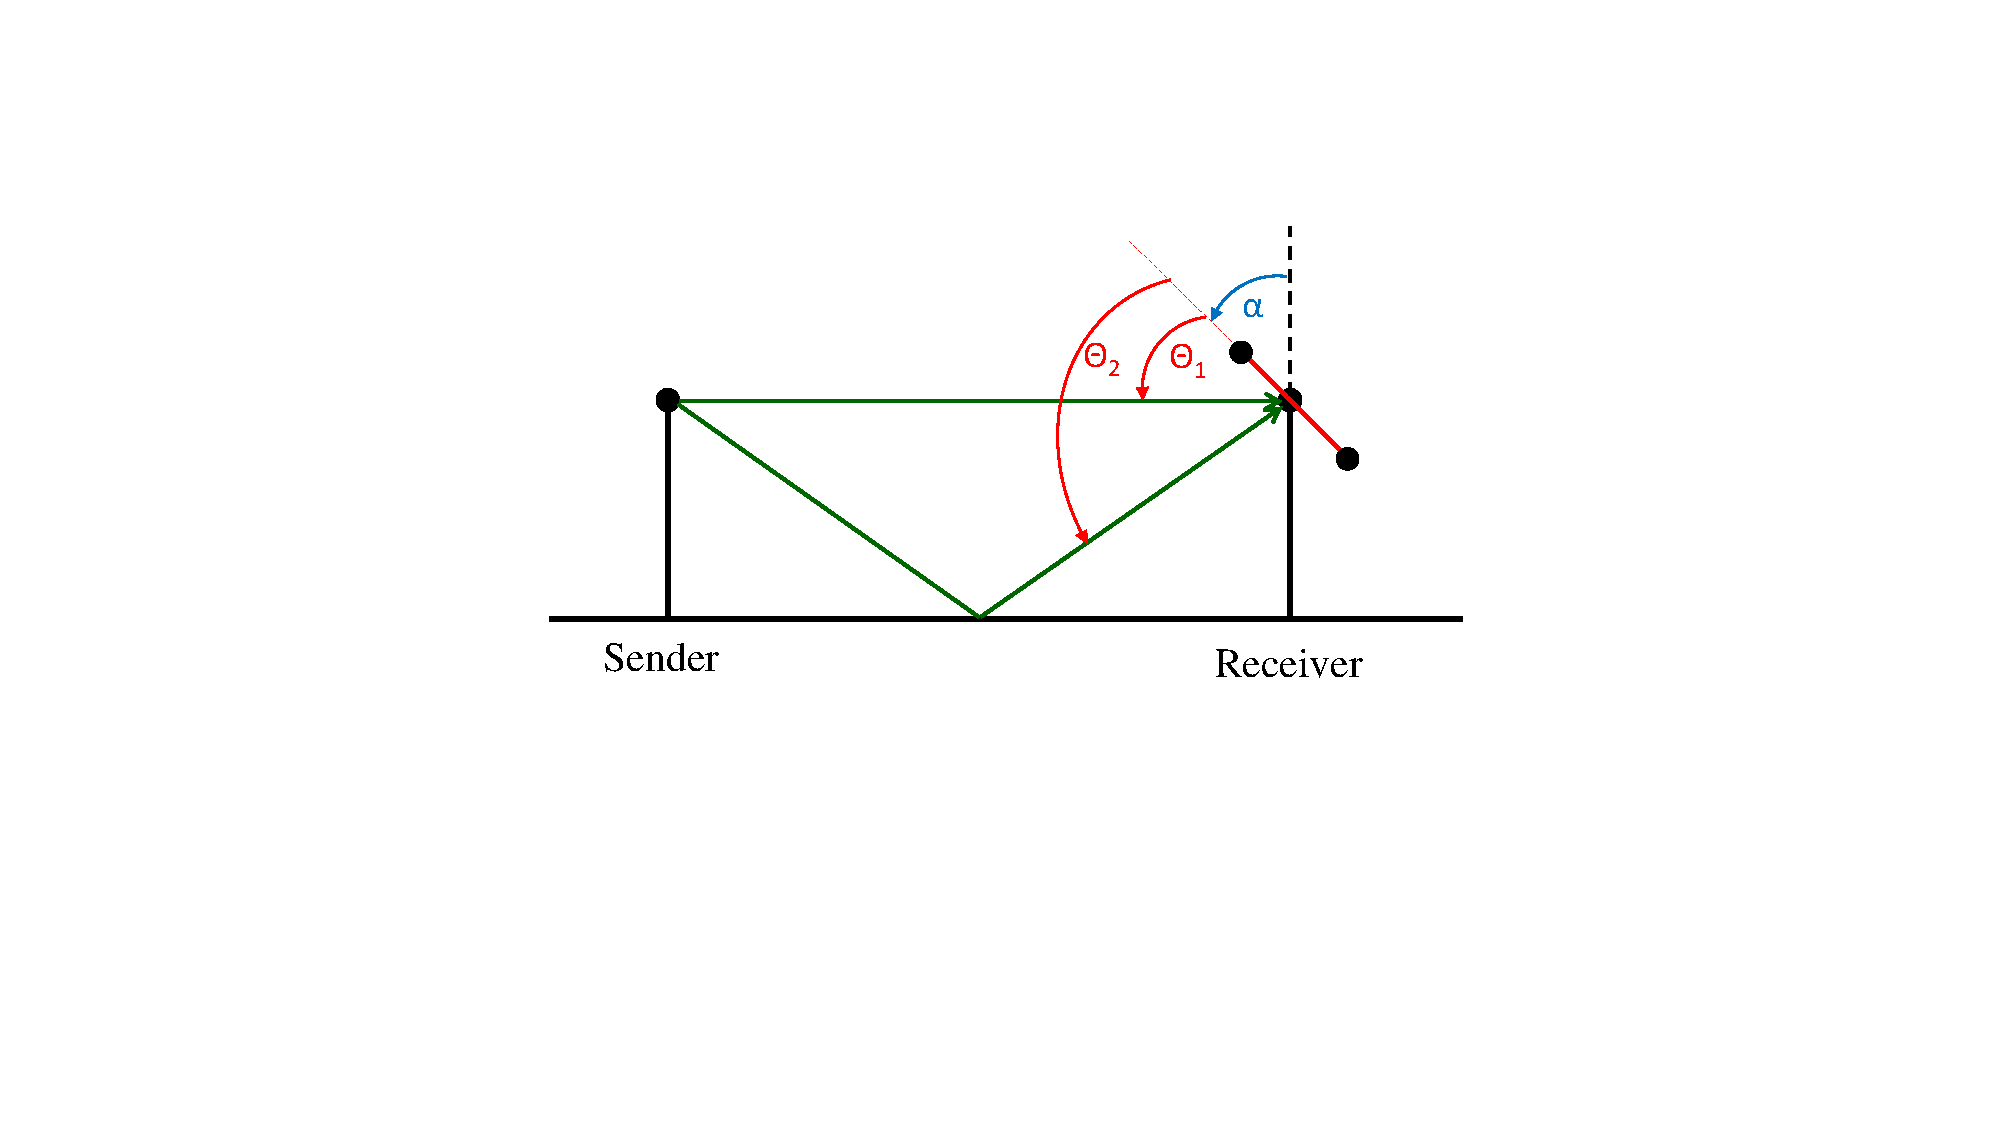
\includegraphics[trim =6cm 7cm 6cm 4cm, clip, width=0.70\textwidth]{graphics/Spatial_filtering_antenna_example_alpha_opt.pdf}
	\caption{Example of a spatial filtering with ULA and tilt angle $\alpha$}
	\label{fig:Spatial_filtering_antenna_example_alpha_opt}
\end{figure}
Choose $\alpha_{opt}$ such that $\vec{a}^H(\Theta_1)\vec{a}(\Theta_2)=0$ (see figure \ref{fig:Spatial_filtering_antenna_example_alpha_opt}).\\
$\ma{A}^H\ma{A}=\mat{\vec{a}^H(\Theta_1)\\\vec{a}^H(\Theta_2)}\mat{\vec{a}(\Theta_1)&\vec{a}(\Theta_2)}=\mat{M&0\\0&M}=M\ma{I}$\\ \\

\textbf{Example:}\\
M=2 \pfeil 2 antennas\\
\begin{figure}[H]
	\centering
		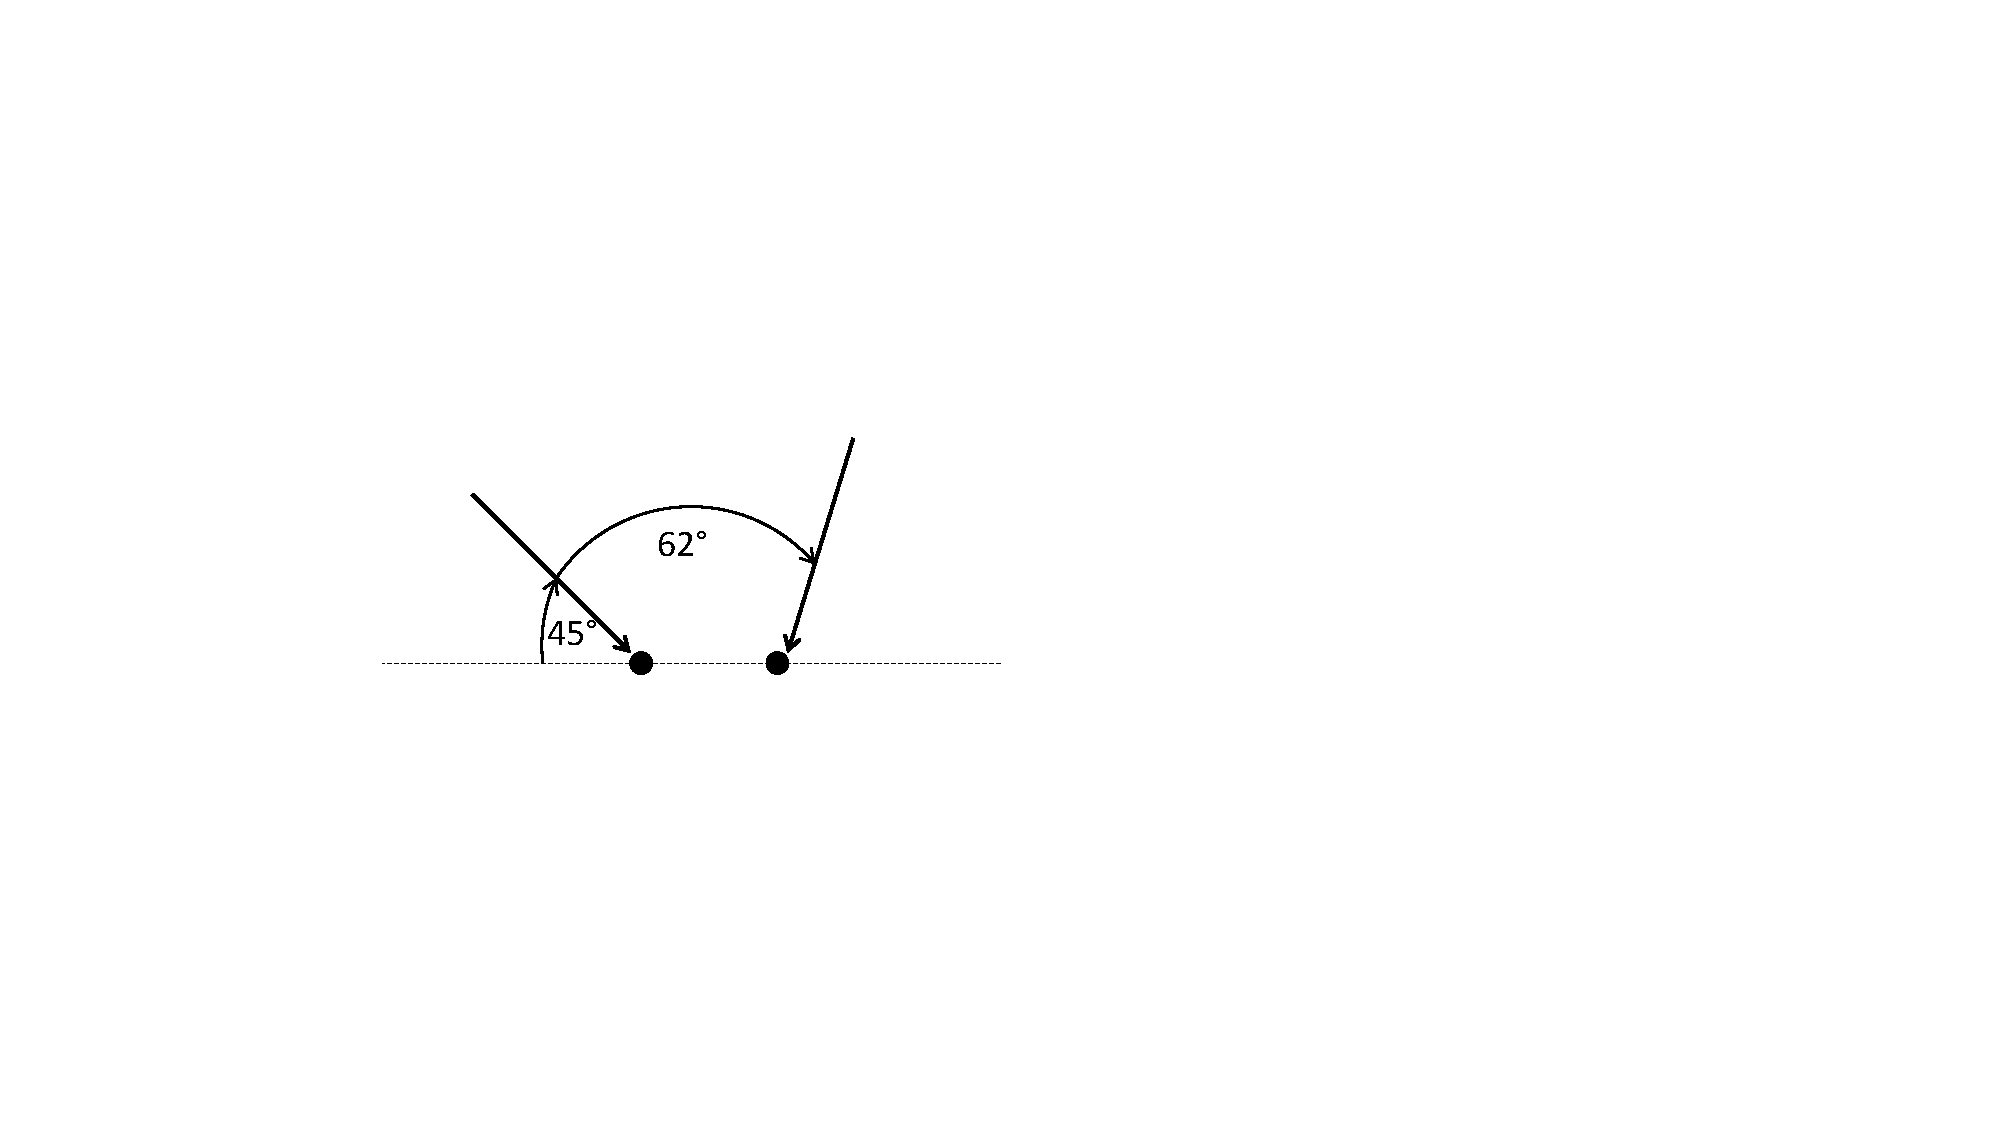
\includegraphics[trim =6cm 7.5cm 14cm 4cm, clip, width=0.50\textwidth]{graphics/LS_filter_example_two_antenna.pdf}
	\caption{Example for $M=2$ and different angles of the arriving signals}
	\label{fig:LS_filter_example_two_antenna}
\end{figure}
$\vec{a}^H(\Theta_1)\vec{a}(\Theta_2)=0$
\end{doublespace}

\subsection{Case 2: Improved Least-Squares - BLUE}
\begin{doublespace}
$\rightarrow$ \textbf{B}est \textbf{L}inear \textbf{U}nbiased \textbf{E}stimator (BLUE)\\
$\ma{X}=\ma{A}\ma{S}+\ma{\nu}$\\
$\ma{W}^H\ma{X}=\underbrace{\ma{W}^H\ma{A}}_{\ma{I}\text{ (unbiased)}}\ma{S}+\underbrace{\ma{W}^H\ma{\nu}}_{\text{Estimation Noise}}$\\
$\ma{W}_{BLUE}=\arg\min\limits_{\ma{W}} E[||\ma{W}^H\ma{\nu}||_F^2],\quad \text{s. t.} \ma{W}^H\ma{A}=\ma{I}_d$\\
\begin{flalign*}
E[||\ma{W}^H\ma{\nu}^H||_F^2]&=E[\trace(\ma{W}^H\ma{\nu}\ma{\nu}^H\ma{W})]
=\trace E[\ma{W}^H\ma{\nu}\ma{\nu}^H\ma{W}]
=\trace(\ma{W}^H \overbrace{E[\ma{\nu}\ma{\nu}^H]}^{N\cdot \ma{R}_\nu}\ma{W})&&\\
&=N\cdot \trace(\ma{W}^H\ma{R}_\nu\ma{W})
\end{flalign*}
$\ma{W}=\mat{\vec{w}_1&\vec{w}_2&\shdots&\vec{w}_d}$\\
$\ma{W}^H\ma{A}=\ma{I}_d \Leftrightarrow\quad \vec{w}_1^H\ma{A}=\vec{e}_1^T,\quad\vec{w}_2^H\ma{A}=\vec{e}_2^T,\quad\ldots,\quad\vec{w}_d^H\ma{A}=\vec{e}_d^T$\\
Lagrange function with equality constraints:\\
$\mathcal{L}=\trace(\ma{W}^H\ma{R}_\nu\ma{W})+2\Re{(\vec{e}_1^T-\vec{w}_1^H\ma{A})\vec{\lambda}_1}+ \ldots + 2\Re{(\vec{e}_d^T-\vec{w}_d^H\ma{A})\vec{\lambda}_d}$\\
$\with \mat{\vec{\lambda}_1 & \vec{\lambda}_2 & \shdots & \vec{\lambda}_d}=:\ma{\lambda}$\\
\begin{flalign*}
\with\trace\left((\ma{I}-\ma{W}^H\ma{A})\ma{\lambda}\right)&=\trace \mat{\vec{e}_1^T-\vec{w}_1^H\ma{A}\\\svdots\\\vec{e}_d^T-\vec{w}_d^H\ma{A}}\mat{\vec{\lambda}_1&\shdots&\vec{\lambda}_d}&&\\
&=(\vec{e}_1^T-\vec{w}_1^H\ma{A})\lambda_1+(\vec{e}_2^T-\vec{w}_2^H\ma{A})\lambda_2+\ldots+(\vec{e}_d^T-\vec{w}_d^H\ma{A})\lambda_d
\end{flalign*}
\begin{flalign*}
\mathcal{L}&=\trace(\ma{W}^H\ma{R}_\nu\ma{W})+2\Re{(\trace(\ma{I}-\ma{W}^H\ma{A})\ma{\lambda}}&&\\
&=\trace(\ma{W}^H\ma{R}_\nu\ma{W})+\trace((\ma{I}-\ma{W}^H\ma{A})\ma{\lambda})+\trace(\ma{\lambda}^H(\ma{I}-\ma{A}^H\ma{W})
\end{flalign*}
$\frac{\partial\mathcal{L}}{\partial\ma{W}^*}=\ma{R}_\nu\ma{W}-\ma{A}\ma{\lambda}\stackrel{!}{=}0 \Rightarrow \ma{W}=\ma{R}_\nu^{-1}\ma{A}\ma{\lambda},\quad \ma{W}^H=\ma{\lambda}^H\ma{A}^H\ma{R}_\nu^{-1}$\\
$\ma{W}^H\ma{A}=\ma{I}=\ma{\lambda}^H\ma{A}^H\ma{R}_\nu^{-1}\ma{A}=\ma{I}$\\
$\ma{\lambda}^H=(\ma{A}^H\ma{R}_\nu^{-1}\ma{A})^{-1}$\\
\mybox{
$\ma{W}_{BLUE}^H=(\ma{A}^H\ma{R}_\nu^{-1}\ma{A})^{-1}\ma{A}^H\ma{R}_\nu^{-1}$
}\\

$\ma{R}_\nu=\const\cdot\ma{I} \Rightarrow \ma{W}_{BLUE}=\ma{W}_{LS}$\pfeil white noise\\
Reconstruction of the signal:\\
$\ma{\hat{S}}=\ma{S}+\ma{W}_{BLUE}^H\ma{\nu}$\\
Calculate SNR:\\
$E[||\ma{W}_{BLUE}^H\ma{\nu}||_F^2]=\trace E[\ma{W}_{BLUE}\ma{\nu}\ma{\nu}^H\ma{W}_{BLUE}]=N\trace (\ma{W}_{BLUE}^H\ma{R}_\nu\ma{W}_{BLUE})$\\
$SNR_{BLUE}=\frac{\trace \ma{R}_s}{\trace (\ma{W}_{BLUE}^H\ma{R}_\nu\ma{W}_{BLUE})}$\\
With: $\ma{W}_{BLUE}^H\ma{R}_\nu\ma{W}_{BLUE}=\underbrace{\underbrace{(\ma{A}^H\ma{R}_\nu^{-1}\ma{A})^{-1}\ma{A}^H\ma{R}_\nu^{-1}}_{\ma{W}_{BLUE}}\underbrace{\ma{R}_\nu\ma{R}_\nu^{-1}}_{\ma{I}}\ma{A}}_{\ma{I}}(\ma{A}^H\ma{R}_\nu^{-1}\ma{A})$\\
\mybox{
$SNR_{BLUE}=\frac{\trace \ma{R}_s}{\trace((\ma{A}^H\ma{R}_\nu^{-1}\ma{A})^{-1})}$\\
}
\mybox{
$SNR_{LS}=\frac{\trace \ma{R}_s}{\trace(\ma{A}^+\ma{R}_\nu(\ma{A}^+)^H)};\qquad \ma{A}^+=(\ma{A}^H\ma{A})^{-1}\ma{A}^H$
}\\ \\
BLUE and LS method are identical if:\\
$\ma{R}_\nu=\const\cdot\ma{I}\quad$ or $\quad M=d \Leftrightarrow SNR_{LS}=SNR_{BLUE}$\\
\Ra\ Only improvement for:
\begin{itemize}
	\item More sensors ($d<M$)
	\item $\ma{R}_\nu\neq\const\cdot\ma{I}$ (no white noise, but colored noise)
\end{itemize}

\subsubsection{Introduction signal correlation matrix as a substitution of the noise correlation matrix}
$\ma{W}_{BLUE}^H =(\ma{A}^H\ma{R}_\nu^{-1}\ma{A})^{-1}\ma{A}^H\ma{R}_\nu^{-1}$\\
\Ra\ We need to know \ma{A} and $\ma{R}_\nu$ or just \ma{A} and allow \emph{latency time}.\\ \\
\textbf{Why can we trade in $\ma{R}_\nu$ for latency time?}\\
$\ma{W}_{BLUE}^H =(\ma{A}^H\ma{R}_x^{-1}\ma{A})^{-1}\ma{A}^H\ma{R}_x^{-1}$\qquad
where $\ma{R}_x=E[\vec{x}[n]\vec{x}^H[n]]$ is the signal correlation matrix\\
The orginal optimization is:\\
$\ma{W}_{BLUE}=\arg\min E[||\ma{W}^H\ma{\nu}||_F^2],\quad \text{s. t. } \ma{W}^H\ma{A}=\ma{I}$\\
Now substitude Noise $\ma{\nu}$ with $\ma{X}$:\\
$\ma{X}=\ma{A}\ma{S}+\ma{\nu}\pfeil$with optimal $\ma{W}^H$ \pfeil $\qquad \ma{W}^H\ma{X}\left.\right|_{\ma{W}^H\ma{A}=\ma{I}}=\ma{S}+\ma{W}^H\ma{\nu}$\\
substitutional optimization:
\begin{flalign*}
E[\ma{W}^H\ma{X}\ma{X}^H\ma{W}]\left.\right|_{\ma{W}^H\ma{A}=\ma{I}}&=E\left[(\ma{S}+\ma{W}^H\ma{\nu})(\ma{S}^H+\ma{\nu}^H\ma{W})\right]&&\\
&\underbrace{=}_{E[\ma{S}\ma{\nu}]=0} E[\ma{S}^H\ma{S}]+\ma{W}^H\ma{R}_\nu\ma{W}
\end{flalign*}
Note: $E[\ma{S}\ma{\nu}]=0$ means that noise and signal are uncorrelated, which can be assumed usually.\\

$\underbrace{\trace{E[\ma{W}^H\ma{X}\ma{X}^H\ma{W}]}}_{E[||\ma{W}^H\ma{X}||_F^2}\left.\right|_{\ma{W}^H\ma{A}=\ma{I}}=\trace(E[\ma{S}\ma{S}^H])+\underbrace{\trace(\ma{W}^H\ma{R}_\nu\ma{W})}_{E[||\ma{W}^H\ma{\nu}||_F^2}$\\
If $\ma{W}\ma{A}=\ma{I}$ is met, then $\min||\ma{W}^H\ma{X}||_F^2$ will minimize $E[||\ma{W}^H\ma{\nu}|_F^2]$ because $\ma{W}^H\ma{X}=\ma{S}\ma{W}^H\ma{\nu}$. $\tr (E[\ma{S}\ma{S}^H]) = \const$\\
So we can exchange $\ma{R}_\nu$ with $\ma{R}_x$.\\
Estimate $\ma{R}_x$ as:
\begin{flalign*}
\ma{\hat{R}}_x=\frac{1}{N}\sum\limits_{k=0}^{N-1}\vec{x}[n+k]\vec{x}^H[n+k]=\frac{1}{N} \ma{X}\ma{X}^H
\end{flalign*}
There is no need to know the noise, but we need to know N snapshots to fill $\ma{X}$. \\\pfeil therefore latency time! \\
\mybox{
$\ma{\hat{W}}_{BLUE}^H=\left(\ma{A}^H\left(\ma{X}\ma{X}^H\right)^{-1}\ma{A}\right)^{-1}\ma{A}^H\left(\ma{X}\ma{X}^H\right)^{-1}$\\
Note: $\ma{\hat{W}}_{BLUE}^H$ needs to be computed before we can use the filter. This causes \emph{latency}.\\
$\ma{\hat{S}}_{BLUE}=\ma{\hat{W}}_{BLUE}^H\ma{X} \rightarrow$ Latency!
}
\mybox{
$\ma{W}_{LS}^H=(\ma{A}^H\ma{A})$\\
$\ma{\hat{S}}_{LS}=\ma{W}_{LS}^H\ma{X} \rightarrow$ No latency!\\
}
\end{doublespace}

\subsection{Case 3: LMMSE-Estimator (Linear Minimum Mean Square Error)}
\begin{doublespace}
$\ma{W}_{LMMSE}=\arg\min\limits_{\ma{W}}\underbrace{E[||\ma{\hat{S}}-\ma{S}||_F^2]}_{J}$\\
$\ma{\hat{S}}=\ma{W}^H\ma{X}$\qquad Estimate Signal Matrix\\

Cost Function:
\begin{flalign*}
J&=E[||\ma{W}^H\ma{X}-\ma{S}||_F^2]&&\\
&=E\left[\trace\left((\ma{W}^H\ma{X}-\ma{S})(\ma{X}^H \ma{W} - \ma{S})\right)\right]&&\\
&=\trace\left(\ma{W}^H E[\ma{X}\ma{X}^H]\ma{W}\right) - \trace\left(\ma{W} E[\ma{X}\ma{S}^H]\right) - \trace\left(E[\ma{S}\ma{X}^H]\ma{W}\right) + \trace\left(E[\ma{S}\ma{S}^H]\right)
\end{flalign*}
Singal Correlation Matrix: \\ $E[\ma{X}\ma{X}^H]=N\ma{R}_x$ \\ 
Channel output Correlation Matrix: \\$E[\ma{S}\ma{S}^H]=N\ma{R}_S$\\ 
Correlation between Signal and Channel Output:\\ $E[\ma{X}\ma{S}^H]=E\left[(\ma{A}\ma{S}-\ma{\nu})\ma{S}^H\right] = \ma{A}E[\ma{S}\ma{S}^H]+E[\ma{\nu}\ma{S}^H]$ \\ 

With assumimg, that noise and signal are uncorrelated ($E[\ma{\nu}\ma{S}^H]=\ma{0}$) we get:\\
$E[\ma{X}\ma{S}^H] = \ma{A}E[\ma{S}\ma{S}^H] = \ma{A}\ma{R}_s N$\\
With the property $\ma{R}_s=\ma{R}_s^H$ (Recall: All correlation matrices are hermitian matrices) we get for our cost function J:\\
$J=N\trace\left(\ma{W}^H\ma{R}_x\ma{W}\right)-N\trace\left(\ma{W}^H\ma{A}\ma{R}_s\right) - N \trace\left(\ma{R}_s\ma{A}^H\ma{W}\right) + N\trace\left(\ma{R}_s\right)$\\ \\
Now what is our filter matrix $\ma{W}_{LMMSE}$?\\
$\frac{\partial J}{\partial \ma{W}^*}=N\ma{R}_x\ma{W}-N\ma{A}\ma{R}_s\stackrel{!}{=}0$\\
\mybox{
$\ma{W}_{LMMSE}=\ma{R}_x^{-1}\ma{A}\ma{R}_s$ 
\qquad or\qquad
$\ma{W}_{LMMSE}^H=\ma{R}_s\ma{A}^H\ma{R}_x^{-1}$
}
\textbf{Derive Correlation Matrices}
\begin{flalign*}
\ma{R}_x&=E[\vec{x}[n]\vec{x}^H[n]]\underbrace{=}_{\text{stationarity}}\frac{1}{N}\sum\limits_{k=0}^{N-1}E[x[n+k]x^h[n+k]]&&\\
&=\frac{1}{N}E[\ma{X}\ma{X}^H]&&\\
&=\frac{1}{N}E\left[(\ma{A}\ma{S}+\ma{\nu})(\ma{A}^H\ma{A}^H+\ma{\nu}^H)\right]; \qquad \ma{X}=\ma{A}\ma{S}+\ma{\nu}&&\\
&=\frac{1}{N}\left(\ma{A}\underbrace{E[\ma{S}\ma{S}^H]}_{N\ma{R}_s}+\ma{A}\underbrace{E[\ma{S}\ma{\nu}^H]}_{\ma{0}}+\underbrace{E[\ma{\nu}\ma{S}^H]}_{\ma{0}}\ma{A}^H+\underbrace{E[\ma{\nu}\ma{\nu}^H]}_{N\ma{R}_\nu}\right)
\end{flalign*}
\mybox{
$\ma{R}_x=\ma{A}\ma{R}_s\ma{A}^H+\ma{R}_\nu$
}
\\ \\
Assueme: \ma{A} has got full column rank \Ra $\ma{A}^+\ma{A}=\ma{I}$ therefore we can obtain $\ma{R}_S$\\
\mybox{
$\ma{R}_s=\ma{A}^+(\ma{R}_x-\ma{R}_\nu)(\ma{A}^+)^H$ \pfeil it's not neccessary to know $\ma{R}_S$
}
\mybox{
\begin{flalign*}
\ma{W}_{LMMSE}^H&=\ma{A}^+(\ma{R}_x-\ma{R}_\nu)(\ma{A}^+)^H\ma{A}^H\ma{R}_x^{-1}&&\\
&=(\ma{A}^H\ma{A})^{-1}\ma{A}^H(\ma{R}_x-\ma{R}_\nu)\ma{A}(\ma{A}^H\ma{A})^{-1}\ma{A}^H\ma{R}_x^{-1}
\end{flalign*}
}
$\ma{\hat{R}}_x=\frac{1}{N}\ma{X}\ma{X}^H \qquad \ma{R}_\nu=\ma{R}_x\left.\right|_{\ma{S}=\ma{0}};$\\
$ \ma{R}_x^{-1}$ has to be regular (squares matrix with det $\neq 0)\pfeil N\geq M$\\
Where $M$ is the number of sensors and $N$ the number of snapshots we take.\\
$\ma{R}_\nu=\frac{1}{N}\ma{X}\ma{X}^H \left.\right|_{\ma{S}=\ma{0}}$

\Ra Possibility: Run BLUE, LS and LMMSE in parallel and choose the one that performes best. Decide on the parameter checksum / error routine which has the least error. 
\end{doublespace}
